\documentclass{iithesis}
\usepackage{polski}
\usepackage[utf8]{inputenc}

\usepackage{amsmath}
\usepackage{amsfonts}

\usepackage{graphicx}
\usepackage{dblfloatfix}
\usepackage{tikz}
\usetikzlibrary{shapes.geometric, arrows}

\usepackage{url}
% \usetikzlibrary{decorations.pathmorphing}

\polishtitle    {Kompaktowe reprezentacje binarne i~modele generatywne}
\englishtitle   {Compact binary representations and generative models}
\polishabstract {Niniejsza praca przedstawia możliwości zastosowania autoenkodera wariacyjnego
                (VAE) do znalezienia reprezentacji (w tym kompatkowej reprezentacji binarnej) dla chmur punktów 3D.
                W~pracy opisano teoretyczne podstawy uczenia autoenkoderów wariacyjnych z~regularyzacją
                zmiennej ukrytej rozkładem normalnym. Przedstawiono również metodę wykorzystywaną do
                wymuszenia bardziej skomplikowanych rozkładów na zmiennej ukrytej
                (m.in. Gamma, Beta oraz mieszanek gaussowskich).
                Opisano również, w~jaki sposób wykorzystać regularyzację mieszanką gaussowską do
                podzielenia danych na naturalne klastry.
                Ponadto zaproponowano sposób użycia VAE z~regularyzację rozkładem Beta do znalezienia kompatkowej
                reprezentacji binarnej dla chmur punktów 3D. Opisane modele zaimplementowano i~przeprowadzono
                szereg eksperymentów sprawdzających ich zdolności rekonstrukcji oraz możliwości generatywne.}
\englishabstract{The following work demonstrates the possibility of using a~variational autoencoder (VAE)
                for obtaining representations (including a~compact binary one) for 3D point clouds.
                The paper includes theoretical baseline study of training variational autoencoders with
                a~normally-distributed latent variable. A~method for regularization of the latent variable
                with a~more complex distribution (such as Gamma, Beta or a~gaussian mixture) has also been presented.
                The work includes also a~description of how to use a~variational autoencoder regularized
                with a~gaussian mixture to divide data into natural clusters.
                Moreover the paper contains a~proposed method of utilising a~Beta-regularized VAE
                in order to obtain a~compact binary representation for 3D point clouds.
                All described models have later been implemented and tested with a~variety of experiments
                focusing on their reconstructive and generative capabilites.}
\advisor        {dr Rafał Nowak}
\author         {Jakub Zadrożny}
\date           {6 września 2019}

\begin{document}

\chapter{Wprowadzenie}
Modele generatywne, takie jak autoenkoder wariacyjny (w skrócie \textbf{VAE}),
stały się obecnie jednym z~podstawowych narzędzi
do pracy z~wielomami rodzajami danych od zdjęć twarzy do plików muzycznych.
Umożliwiają one znajdowanie efektywnych i~interpretowalnych reprezentacji, które
pozwalają nie tylko na generowanie syntetycznych danych, ale rozwiązują również problemy takie
jak gładka inerpolacja pomiędzy dwoma obiektami, czy edycja obiektów poprzez intuicyjne operacje.

Obecnie jednak, dzięki popularyzacji urządzeń reprezentujących głębię obrazu,
takich jak LIDAR i~kamera RGB-D, coraz większą rolę odgrywają chmury punktów 3D.
Wykorzystuje się je w~wielu nowoczesnych, rewolucyjnych i~kluczowych dla postępu technologiach,
m.in. pojazdach autonomicznych, robotyce oraz wirtualnej i~rozszerzonej rzeczywistości.
Chmury punktów są dość skomplikowanymi danymi, które zajmują znacznie ilości miejsca i~przetwarzane
w oryginalnej postaci nakładają spory narzut obliczeniowy. Dlatego istotnym zagadnieniem
jest znalezienie odpowiedniej reprezentacji dla takich danych. Taka reprezentacja
musi być kompaktowa, aby zmniejszyć narzut pamięciowy i~obliczeniowy, a~model powininen być generatywny,
żeby umożliwić tworzenie i~edycję obiektów.

Chmury punktów 3D są aktywnym obszarem badań i~na przestrzeni ostatnich lat powstało zarówno
wiele problemów (np. zbiory ShapeNet \cite{shapenet} i~ModelNet40 \cite{modelnet}), jak i
rozwiązań (np. architektura PointNet \cite{pointnet} i~metryka EMD \cite{emd}).
Niektóre z~tych osiągnięć pozwalają tworzyć kolejne, bardziej zaawansowane modele,
m.in. opisany w~tej pracy autoenkoder wariacyjny, który na podstawie znalezionej reprezentacji
potrafi rekonstruować i~generować nowe chmury punktów.

Jednym ze znanych problemów VAE, jest trudność narzucenia na zmienną ukrytą niektórych mniej typowych rozkładów.
W~dalszej części pracy opisano znane rozwiązania tego problemu, rozszerzające możliwości enkodera,
dzięki którym da się regularyzować zmienną ukrytą np. rozkładem Gamma, Beta oraz mieszanką gaussowską.
Wykazano również, w~jaki sposób wykorzystać regularyzację reprezentacji mieszanką gaussowską,
aby podzielić dane na naturalne klastry, zgodnie z~ich cechami charakterystycznymi, w~sposób w~pełni nienadzorowany.
Dodatkowo podano metodę, która pozwala wykorzystać VAE do znalezienia kompaktowej reprezentacji binarnej.
Wykorzystanie takiej reprezentacji pozwala rozwiązać kluczowy w~dobie
wszechobecnych danych problem -- można drastycznie ograniczyć ilość przechowywanych i~przetwarzanych informacji.
Uzyskana reprezentacja zajmuje jedynie 128 bitów na jedną chmurę, co przy prawie 200kb w~oryginalnej
reprezentacji daje ponad 1500-krotną skalę kompresji.
Ponadto reprezentacja binarna zawiera tyle informacji, ile zaledwie czterowymiarowa
reprezentacja ciągła, jednak posiada większą zdolność rekonstrukcji, nie poświęcając
przy tym możliwości generatywnych.

Podsumuwując, praca składa się z~czterech głównych części: (1) zawiera opis teoretycznych podstaw
autoenkodera wiaracyjnego, (2) podaje sposoby wymuszenia różnych rozkładów na zmiennej ukrytej,
(3) zawiera eksperymenty demonstrujące zdolności wytrenowanego modelu do rekonstrukcji,
generowania syntetycznych danych, interpolacji, edycji obiektów przez intuicyjne operacje oraz klasteryzacji
i (4) opsiuje sposób, w~jaki można wykorzystać VAE z~regularyzacją rozkładem Beta do otrzymania
kompaktowej (128 bitów) reprezentacji binarnej chmur punktów i~potwierdza skuteczność tej
reprezentacji eksperymentami.

\chapter{Podstawy opracowania}

\section{Chmury punktów 3D} \label{sec:point_clouds}
Chmury punktów 3D reprezentują obiekty, kształty, powierzchnie w~przestrzeni za pomocą zbioru
trójek liczb rzeczywistych: współrzędnych $x,y,z$ każdego z~punktów.
Pojedynczą chmurę punktów reprezentuje zatem macierz wymiaru $3 \times N$,
gdzie $N$ -- liczba punktów. Ponieważ chmury reprezentowane są przez \textit{zbiór} punktów,
przyjmujemy, że dwie macierze różniące się tylko kolejnością kolumn
przedstawiają w~rzeczywistości tę samą chmurę. Stwarza to dwa istotne problemy: (1) cały model powinien
być niewrażliwy na permutacje kolumn macierzy wejściowej, (2) dekoder trzeba oceniać metryką niewrażliwą
na permutacje punktów.

\subsubsection{Architektura PointNet}
Silnym narzędziem do pracy z~chmurami punktów 3D jest architektura \textbf{PointNet} \cite{pointnet},
która umożliwa ekstrakcję cech (w pełni sparametryzowanych) z~wejściowej chmury punktów.
Architektura ta posiada dwie podstawowe zalety istotne dla tej pracy: jest odporna na permutacje
punktów chmury wejściowej i~przyjmuje jako wejście chmury w~naturalnej postaci.
Inne metody \cite{voxnet,modelnet} rozwiązały problem permutacji przetwarzając
chmury punktów na inne formaty (np. wykorzystujące voxele), przez co rozmiar przetwarzanych
danych i~czas obliczeń wzrasta. PointNet osiąga ten sam cel, zachowując
względną prostotę modelu, co z~uwagi na ograniczone zasoby obliczniowe jest kluczowe.

\subsubsection{Metryki}
Powszechnie stosuje się dwie metryki dla chmur punktów 3D; zob. np. \cite{metrics}.
Załóżmy, że dysponujemy dwoma zbiorami $S_1 \in \mathbb{R}^3$ i~$S_2 \in \mathbb{R}^3$.

Metryka \textit{Chamfer} pseudo-distance (\textbf{CD}) dla każdego punktu z~$S_1$ oblicza
odległość od najbliższego punktu w~$S_2$ i~odwrotnie. Dana jest następującym wzorem:
\begin{equation} \label{eq:chamfer_intro}
CD(S_1, S_2) = \sum_{x \in S_1} \min_{y \in S_2} ||x-y||_2^2 + \sum_{y \in S_2} \min_{x \in S_1} ||x-y||_2^2.
\end{equation}

Metryka Earth-mover distance (\textbf{EMD}) \cite{emd} znajduje permutację punktów wyjściowego zbioru,
dla której suma odległości punkt po punkcie jest najmniejsza. Dana jest wzorem:
\begin{equation}
EMD(S_1, S_2) = \min_{\phi:S_1 \rightarrow S_2} \sum_{x \in S_1} ||x-\phi(X)||_2^2,
\end{equation}
gdzie $\phi$ jest bijekcją.

Jak zaznaczają autorzy \cite{pc_representations}, użycie metryki EMD pozwala uzyskać lepsze rezultaty
w rekonstrukcji obiektów, jednak jej wyliczanie jest znacznie bardziej kosztowne niż CD, dlatego
w tej pracy skupiono się na metryce CD.

\section{Autoenkodery}
Podstawowym modelem opisywanem w~tej pracy jest autoenkoder \cite{autoencoders}. Autoenkoder to model
złożony z~dwóch sieci neuronowych: \textbf{enkodera} i~\textbf{dekodera}. Sieci trenuje
się wspólnie, w~taki sposób, aby na podstawie wyniku zwróconego przez enkoder, dekoder był w~stanie
zrekonstruować oryginalne dane (wejście do enkodera). Autoenkodery stają się praktyczne, gdy
nałoży się ograniczenie na dane przekazywane pomiędzy enkoderem i~dekoderem
(nazywane zmienną ukrytą lub reprezentacją),
np. ograniczy się mocno ich wymiar. Schemat działania enkodera przedstawia rys. \ref{fig:ae_basics}.

\begin{figure}[b]
    \center{
        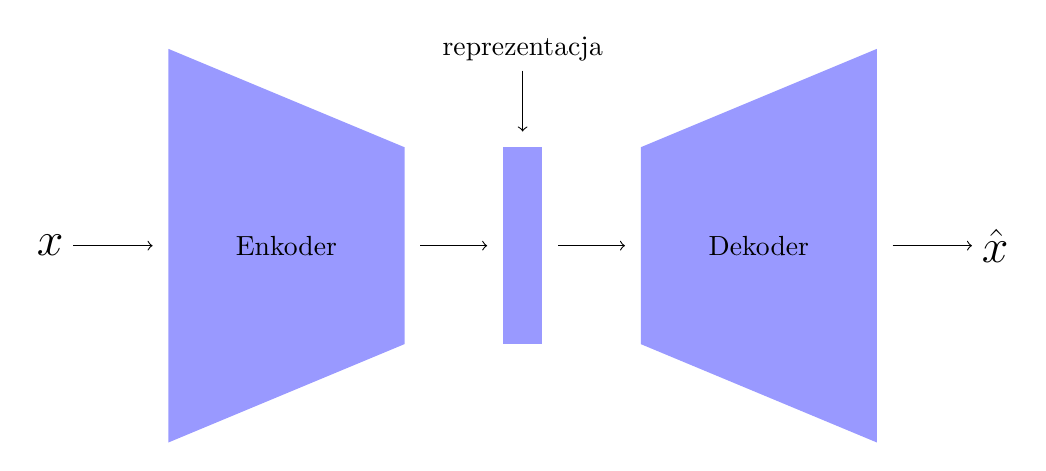
\begin{tikzpicture}
            \fill[blue!40!white] (-4.5,2.5) -- (-4.5,-2.5) -- (-1.5,-1.25) -- (-1.5,1.25) -- cycle;
            \node[inner sep=0pt] at (-3,0) {Enkoder};
            \fill[blue!40!white] (1.5,1.25) -- (1.5,-1.25) -- (4.5,-2.5) -- (4.5,2.5) -- cycle;
            \node[inner sep=0pt] at (3,0) {Dekoder};
            \fill[blue!40!white] (-0.25,1.25) -- (-0.25,-1.25) -- (0.25,-1.25) -- (0.25,1.25) -- cycle;
            \draw[->] (-1.3,0) -- (-0.45,0);
            \draw[->] (0.45,0) -- (1.3,0);
            \node[] at (-6,0) (input) {\LARGE $x$};
            \draw[->] (input) -- (-4.7,0);
            \node[] at (6,0) (output) {\LARGE $\hat{x}$};
            \draw[->] (4.7,0) -- (output);
            \node[] at (0,2.5) (repr) {reprezentacja};
            \draw[->] (repr) -- (0,1.45);
        \end{tikzpicture}
    }
    \caption{\label{fig:ae_basics} Schemat działania autoenkodera. Celem jest minimalizacja odległości
    pomiędzy $\hat{x}$ i~$x$.}
\end{figure}

\section{Modele generatywne}
Klasycznym wynikiem, który spopularyzował modele generatywne, jest autoenkoder wariacyjny
(\textbf{VAE}) \cite{vae}. Jego najważniejszą zaletą jest probabilistyczny charakter,
dzięki czemu możemy żądać, aby zmienna ukryta (reprezentacja) była zradnomizowana i~pochodziła
z pewnego zadanego rozkładu prawdopodobieństwa (z pewnymi ograniczeniami).
Dzięki randomizacji zmiennych ukrytych uzyskujemy zagęszczenie przestrzeni reprezentacji,
przez co niemal każdy punkt może zostać zdekodowany na realistyczne dane.
Umożliwia to realizowanie zadań takich jak generowanie syntetycznych,
realistycznych danych lub gładkie interpolacje znaczeniowe obiektów.

Modele generatywne są szeroko zbadane i~często stosowane do różnych problemów, m.in. analizy obrazów.
W przypadku chmur punktów 3D ich możliwości i~szczegóły zastosowania są mniej znane.
Jedne z~pierwszych opracowań tego tematu można znaleźć w~\cite{pc_representations}
(autorzy wykorzystują zwykły autoenkoder do znalezienia reprezentacji,
na której uczą modele generatywne -- m.in. model mieszanek gaussowskich oraz GANy \cite{gan})
i~\cite{adversarial} (praca skupia się na zastosowaniu autoenkoderów generatywnych: VAE oraz
autoenkodera przeciwstawnego wykorzystywanego do wymuszenia ciekawszych rozkładów na zmiennej ukrytej).

\subsubsection{Klasyfikacja i~klasteryzacja}
Modele generatywne można również zaadaptować do celów najczęsciej rozwiązywanych
z użyciem tradycyjnych metod -- klasyfikacji i~klasteryzacji. W~pracy \cite{m2}
zaproponowano modyfikację autoenkodera wariacyjnego, dzięki której mógłby on pełnić rolę
klasyfikatora trenowanego w~sposób pół-nadzorowany (model M2). Chociaż podejście
to zawodzi, gdy zastosuje się je w~sposób całkowicie nienadzorowany, to w~literaturze \cite{gmvae,real_gmvae} można
znaleźć dodatkowe modyfikacje, które umożliwiają modelowi M2 klasteryzację danych w
sposób nienadzorowany. W~dalszej części pracy opisano dokładnie model oparty na autoenkoderze
wariacyjnym, który potrafi dzielić dane na naturalne podkategorie.
% i~inne, np edycja i~uzupelnianie

\section{Estymacja gradientu wartości randomizowanych}
Do wytrenowania autoenkodera wariacyjnego używa się najczęściej wariantu metody
\textit{stochastic gradient descent} (\textbf{SGD}), która wymaga wyliczania pochodnych
funkcji kosztu po kolejnych parametrach modelu, co z~kolei wymaga wyliczania pochodnych
wartości pojawiających się we wszystkich warstwach po parametrach wartstw poprzednich (propagacja wstecz).
Do wyliczenia funkcji kosztu w~VAE używa się szacowania Monte Carlo, które opiera się na
próbkowaniu zmiennej losowej. Oznacza to, że do wytrenowania autoenkodera wariacyjnego
niezbędne jest obliczanie pochodnych wylosowanej zmiennej po parametrach rozkładu.
W~tym celu stosouje się dwie postawowe metody.

Estymator \textbf{score function} opisany m.in. w~\cite{score_fn} oferuje stosunkowo
proste przybliżenie gradientu funkcji kosztu i~można go stosować do szerokiej gamy rozkładów,
jednak charakteryzuje się dużą wariancją oszacowania, co komplikuje proces trenowania.

Drugim podejściem jest \textbf{pathwise gradients}, czyli tzw. trik repearametryzacyjny
opsisywany m.in. w~\cite{vae}. Metoda ta opiera się na przedstawieniu zmiennej $z$~pochodzącej
z rozkładu $q_\theta(z)$, sparametryzowanego przez $\theta$, jako $z=\mathcal{T}(\epsilon;\theta)$,
gdzie $\epsilon$~pochodzi z~pewnego rokładu $q_0$~niezależnego od
$\theta$,~a~$\mathcal{T}$ jest obliczalnym i~różniczkowalnym po $\theta$ przekształceniem.
Trik repearametryzacyjny jest łatwy do zastosowania dla części rozkładów ciągłych
(szczególnie dla tych z~rodziny kształtu i~skali), jednak z~uwagi na brak prostego przekształcenia
$\mathcal{T}$,~nie da się go wprost zastosować do niektórych istotnych rozkładów, np. Gamma i~Beta.

Rozszerzenie tej metody na kolejne rodziny rozkładów zostało zaproponowane w~\cite{pathwise_gradients}.
Wprowadzona metoda, wymaga jedynie istnienia pochodnej dystrybuanty po parametrach
rozkładu w~postaci zwartej lub znalezienia jej dobrego przybliżenia numerycznego.
Mimo niewielkich wymagań, rozwiązanie pozwala w~efektywny sposób szacować gradienty funkcji kosztu,
nawet gdy zmienne pośrednie pochodzą ze skomplikowanych rozkładów jak Gamma i~Beta.

\chapter{Metody} \label{sec:methods}
\section{Autoenkoder wariacyjny z~rozkładem normalnym}
\label{sec:vae_normal}
Możliwości i~metodyka pracy z~autoenkoderami wariacyjnymi jest szeroko zbadana
pod kątem niektórych zagadnień, m.in. analizy obrazów.
Jednak zastosowanie ich do stosunkowo nowych danych, jakimi są chmury punktów 3D,
wymaga opracowania dokładniejszej metody.

Dalej zakładamy, że dysponujemy zbiorem
$$
\mathcal{X} = \{x_i \in \mathbb{R}^{d}\}_{i \in I}
$$
dla pewnego $d$ -- wymiaru danych oraz $I$ -- zbioru indeksów.
Ponadto zakładamy, że dane z~tego zbioru są obserwacjami
zmiennej losowej o~rozkładzie następującej postaci
\begin{equation} \label{eq:generative_process_factorization}
f_\theta(z, x) = f(z)f_\theta(x|z),
\end{equation}
gdzie $z \in \mathbb{R}^k$ dla pewnego $k$ -- zmienna ukryta (\textit{latent}) o~wymiarze $k$,
$x \in \mathbb{R}^d$ -- zmienna obserwowana o~wymiarze $d$, a~$\theta$ -- parametry rozkładu.

Dodatkowo niech
\begin{equation} \label{eq:generative_process_distribs}
\begin{split}
z &\sim \mathcal{N}(0, I_k), \\
x|z &\sim \mathcal{N}(\mu_x(z; \theta), \mu_\sigma(z;\theta)I_d),
\end{split}
\end{equation}
gdzie $\mu_x,\,\mu_{\sigma}$ są skomplikowanymi obliczeniami
wykonywanymi przez sieć neuronową sparametryzowaną przez $\theta$.

\subsection{ELBO} \label{sec:elbo}
Naszym celem jest odtworzenie parametrów $\theta$ rozkładu generującego
oraz rozkładu $f_\theta(z|x)$, który wyznacza reprezentację danych
generowanych przez proces opsiany w
(\ref{eq:generative_process_factorization}) i~(\ref{eq:generative_process_distribs}).

Niestety z~powodu zastosowania skomplikowanych, nieliniowych
transformacji dokładne odtworzenie rozkładu $f_\theta(z|x)$ jest niemożliwe.
W~tym celu wprowadzamy pewne przybliżenie tego rozkładu -- nazwijmy je
$g_\phi(z|x)$. Niech $g_\phi(z|x)$ będzie gęstością
rozkładu normalnego ze średnią $\rho_x(x;\phi)$ i~wariancją $\rho_\sigma(x;\phi)$,
gdzie $\rho_x,\rho_\sigma$ są reprezentowane przez sieci neuronowe parametryzowane przez $\phi$.

%Będzie to rozkład pochodzący z~pewnej ustalonej rodziny, sparametryzowany przez $\phi$.

Dla ustalonego $x$ mamy
\begin{equation*}
\begin{split}
KL(g_\phi(z|x) || f_\theta(z|x)) &= \mathbb{E}_{z \sim g_\phi(z|x)}\left[
-\log\frac{f_\theta(z|x)}{g_\phi(z|x)}\right] \\
&=\mathbb{E}_{z\sim g_\phi(z|x)}\left[-\log\frac{f_\theta(z|x)f_\theta(x)}{g_\phi(z|x)f_\theta(x)}\right] \\
&=\mathbb{E}_{z\sim g_\phi(z|x)}\left[-\log\frac{f_\theta(z|x)f_\theta(x)}{g_\phi(z|x)}+\log f_\theta(x)\right] \\
&=\mathbb{E}_{z\sim g_\phi(z|x)}\left[-\log\frac{f_\theta(z,x)}{g_\phi(z|x)}\right] +\log f_\theta(x),
\end{split}
\end{equation*}
gdzie $KL(\cdotp || \cdotp)$ jest odległością Kullbacka-Leiblera \cite{kl-cost}.
Zatem
\begin{equation*}
\log f_\theta(x) = KL(g_\phi(z|x) || f_\theta(z|x)) +
\mathbb{E}_{z \sim g_\phi(z|x)}\left[\log\frac{f_\theta(z,x)}{g_\phi(z|x)}\right].
\end{equation*}
Ponieważ $KL(\cdotp || \cdotp) \geq 0$, więc
\begin{equation} \label{eq:elbo}
\begin{split}
\log f_\theta(x)  &\geq \mathbb{E}_{z \sim g_\phi(z|x)}\left[\log\frac{f_\theta(z,x)}{g_\phi(z|x)}\right] \\
&= \mathbb{E}_{z \sim g_\phi(z|x)}\left[\log\frac{f_\theta(x|z)f(z)}{g_\phi(z|x)}\right] \\
&=\mathbb{E}_{z \sim g_\phi(z|x)}\left[\log f_\theta(x|z)\right] -
\mathbb{E}_{z \sim g_\phi(z|x)}\left[-\log\frac{f(z)}{g_\phi(z|x)}\right] \\
&=\mathbb{E}_{z\sim g_\phi(z|x)}\left[\log f_\theta(x|z)\right] - KL(g_\phi(z|x) || f(z)).
\end{split}
\end{equation}
Zatem dla dowolnego rozkładu aproksymującego $g_\phi(z|x)$ otrzymujemy dolne
ograniczenie na prawdopodobieństwo wygenerowania zaobserwowanych danych.
Dlatego część wzoru po prawej stronie od ostatniej równości
nazywamy \textit{evidence lower bound} (w skrócie \textbf{ELBO}).

Możemy zauważyć, że ostateczna postać wzoru (\ref{eq:elbo})
składa się z~dwóch części naturalnie odpowiadającymi dwóm
celom, które chcemy zoptymalizować: pierwszy składnik odpowiada
jakości rekonstrukcji obserwacji ze zmiennej ukrytej $z$
(dlatego nazywany jest kosztem rekonstrukcji),
natomiast drugi to odległość KL rozkładu aproksymującego
$f_\theta(z|x)$ od naszego założenia na jego temat.

\subsection{Zadanie optymalizacyjne} \label{sec:optim_task}
Chcemy znaleźć układ parametrów $<\theta,\phi>$, który daje najlepszą
gwarancję na prawdopodobieństwo wygenerowania zaobserwowanych danych (ELBO).
W~tym celu posłużymy się lekko zmodyfikowanym algorytmem SGD.
Niech
\begin{equation} \label{eq:loss_f}
\mathcal{L}(x,\theta,\phi) =
\underbrace{\mathbb{E}_{z\sim g_\phi(z|x)}\left[\log f_\theta(x|z)\right]}_{\mathcal{L}_{rec}(x,\theta,\phi)} -
KL(g_\phi(z|x)||f(z)).
\end{equation}
Korzystając z~(\ref{eq:elbo}) dla każdej pary $\theta,\phi$ mamy
\begin{equation*}
\log \prod_{x \in \mathcal{X}} f_\theta(x) = \sum_{x \in \mathcal{X}} \log f_\theta(x) \geq
\sum_{x \in \mathcal{X}} \mathcal{L}(x,\theta,\phi) \overset{\mathrm{def}}{=} \hat{\mathcal{L}}(\mathcal{X},\theta,\phi).
\end{equation*}
Naszym zadaniem jest znalezienie $\hat{\theta},\hat{\phi}$, takich że
\begin{equation*}
\hat{\mathcal{L}}(\mathcal{X},\hat{\theta},\hat{\phi}) = \max_{\theta,\phi} \hat{\mathcal{L}}(\mathcal{X},\theta,\phi).
\end{equation*}
Ponieważ bardziej naturalnym zadaniem jest minimalizowanie funkcji kosztu,
więc rozwiążemy równoważne zadanie znalezienia $\hat{\theta},\hat{\phi}$, takich że
\begin{equation*}
-\hat{\mathcal{L}}(\mathcal{X},\hat{\theta},\hat{\phi}) = \min_{\theta,\phi} -\hat{\mathcal{L}}(\mathcal{X},\theta,\phi).
\end{equation*}

Aby posłużyć się algorytmem SGD, musimy umieć wyliczać i~różniczkować
oba składniki funckji kosztu $\mathcal{L}$ (zob. \ref{eq:loss_f}).

\subsection{Koszt KL}
Odległość KL dwóch rozkładów normalnych o~następujących parametrach
\begin{equation*}
\begin{split}
\mathcal{N}_0 \sim \mathcal{N}(\mu_0, \Sigma_0), \\
\mathcal{N}_1 \sim \mathcal{N}(\mu_1, \Sigma_1)
\end{split}
\end{equation*}
dla pewnych $\mu_0,\,\mu_1 \in \mathbb{R}^k,\ \Sigma_0, \Sigma_1 \in \mathbb{R}^{k \times k}$, wynosi
\begin{equation*}
KL(\mathcal{N}_0||\mathcal{N}_1) = \frac{1}{2} \left(\text{tr}(\Sigma_1^{-1}\Sigma_0)
+ (\mu_1-\mu_0)^T \Sigma_1^{-1} (\mu_1-\mu_0) -k + \log\frac{\det\Sigma_1}{\det\Sigma_0} \right).
\end{equation*}
Ponieważ zakładamy, że $f(z)$ jest rozkładem $z \sim \mathcal{N}(0, I_k)$, więc
\begin{equation}
KL(g_\phi(z|x) || f(z)) = \frac{1}{2}\sum_{i=1}^k
\left( \rho_x(x;\phi)_i^2 + \rho_\sigma(x;\phi)_i^2 - 2\log(\rho_\sigma(x;\phi)_i)-1 \right).
\label{eq:kl_loss}
\end{equation}
Wzór (\ref{eq:kl_loss}) można wyliczać i~różniczkować analitycznie.

\subsection{Koszt rekonstrukcji} \label{sec:rec_loss_normal}
Drugiego składnika funckji $\mathcal{L}$, czyli kosztu rekonstrukcji $\mathcal{L}_{rec}$,
nie da się wyznaczyć analitycznie. Aby objeść ten problem, możemy metodą Monte Carlo
oszacować wartość oczekiwaną przez średnią:
\begin{equation*}
-\mathcal{L}_{rec}(x,\theta,\phi) = \mathbb{E}_{z \sim g_\phi(z|x)}\left[-\log f_\theta(x|z)\right] \approx
\frac{1}{m} \sum_{i=1}^m -\log f_\theta(x|z_i),
\end{equation*}
gdzie $z_i$ są obserwacjami rozkładu $g_\phi(z|x)$. Taką wartość potrafimy już wyliczyć, ale nie
potrafimy propagować gradientu do parametrów $\phi$ przez
zaobserwowane wartości~$z_i$.

Wprowadzimy reparametryzację zmiennych $z_i$ -- możemy zauważyć, że zmienna
$z_i=\rho_x(x;\phi)+\epsilon_i\rho_\sigma(x;\phi)$
gdzie $\epsilon_i \sim \mathcal{N}(0, I_k)$
ma rozkład $g_\phi(z|x)$, a~ponadto możemy różniczkować $z_i$ po $\rho_x(x;\phi),\rho_\sigma(x;\phi)$
i propagować gradient wstecz do parametrów $\phi$.
Otrzymaliśmy zatem następujące przybliżenie:
$$
-\mathcal{L}_{rec}(x,\theta,\phi) \approx
\frac{1}{m} \sum_{i=1}^m -\log f_\theta(x|z_i=\rho_x(x;\phi)+\epsilon_i\rho_\sigma(x;\phi)),
$$
gdzie $\epsilon_i \sim \mathcal{N}(0, I_k)$. Dalej, dla uproszczenia, przyjmujemy $m=1$.

Niech
\begin{equation*}
\begin{aligned}[t]
x =
\begin{bmatrix}
x_1 \\
\vdots \\
x_d
\end{bmatrix}
\end{aligned}
,\qquad \qquad
\begin{aligned}[t]
\mu_x(z;\phi) =
\begin{bmatrix}
\mu_1 \\
\vdots \\
\mu_d
\end{bmatrix}
.
\end{aligned}
\end{equation*}
Ponadto, dla uproszczenia, zakładamy, że
\begin{equation*}
\mu_\sigma(z;\theta) =
\begin{bmatrix}
\alpha \\
\vdots \\
\alpha
\end{bmatrix}
\overset{\mathrm{def}}{=} \hat{\alpha}
\end{equation*}
dla wszystkich $z$ i~niezależnie od parametrów $\theta$ (tzn. przyjęto stałą wariancję dla danych wyjściowych).

Ponieważ $x|z \sim \mathcal{N}(\mu_x(z;\theta), \alpha I_d)$, więc
\begin{equation} \label{eq:log_density}
-\log f_\theta(x|z)=\sum_{i=1}^d \left( \frac{1}{2}\log(2\pi) + \log \alpha
+\frac{(x_i-\mu_i^2)}{2\alpha} \right).
\end{equation}
Jednak metryka ta niezbyt dobrze nadaje się do chmur punktów,
ponieważ jest zależna od kolejności występowania punktów na wejściu i~wyjściu.

Zarówno dane wejściowe $x$, jak i~wyjściowe $\mu_x(z;\theta)$ możemy potraktować
jak chmury punktów w~$\mathbb{R}^3$, tj.
\begin{equation*}
\begin{aligned}[t]
x =
\begin{bmatrix}
x_{1,1} & & x_{i,1} & & x_{d',1} \\
x_{1,2} & \dots & x_{i,2} & \dots & x_{d',2} \\
x_{1,3} & & x_{i,3} & & x_{d',3}
\end{bmatrix}
\end{aligned}
,\qquad
\begin{aligned}[t]
\mu_x(z;\phi) =
\begin{bmatrix}
\mu_{1,1} & & \mu_{i,1} & & \mu_{d',1} \\
\mu_{1,2} & \dots & \mu_{i,2} & \dots & \mu_{d',2} \\
\mu_{1,3} & & \mu_{i,3} & & \mu_{d',3}
\end{bmatrix}
,
\end{aligned}
\end{equation*}
gdzie $d'=\frac{d}{3}$. Dodatkowo niech
\begin{equation*}
\begin{aligned}[t]
x_i =
\begin{bmatrix}
x_{i,1} \\
x_{i,2} \\
x_{i,3}
\end{bmatrix}
\end{aligned}
,\qquad \qquad
\begin{aligned}[t]
\mu_i =
\begin{bmatrix}
\mu_{i,1} \\
\mu_{i,2} \\
\mu_{i,3}
\end{bmatrix}
.
\end{aligned}
\end{equation*}
Wtedy równanie (\ref{eq:log_density}) można zapisać jako
\begin{equation} \label{eq:modified_log_density}
-\log f_\theta(x|z)=\sum_{i=1}^{d'} \left( \frac{3}{2}\log(2\pi) + 3\log \alpha
+\frac{||x_i-\mu_i||_2^2)}{2\alpha} \right).
\end{equation}

Aby uzyskać niewrażliwość funkcji kosztu na permutacje punktów wejściowych i~wyjściowych
za koszt rekonstrukcji przyjmiemy
\begin{equation} \label{eq:final_rec_loss}
\begin{split}
-\mathcal{L'}_{rec}(x,\theta,\phi) &= \frac{1}{2\alpha} \left( \sum_{i=1}^{d'} \min_{j=1}^{d'} ||x_i-\mu_j||^2_2
+ \sum_{i=1}^{d'} \min_{j=1}^{d'} ||\mu_i-x_j||^2_2 \right) \\
&= \frac{1}{2\alpha} CD(S_1,S_2),
\end{split}
\end{equation}
gdzie $S_1 = \{x_i \,|\, 1 \leq i~\leq d'\}$ i~$S_2 = \{\mu_i \,|\, 1 \leq i~\leq d'\}$,
a $CD$ dane jest wzorem (\ref{eq:chamfer_intro}).

Możemy zauważyć, że wzór (\ref{eq:final_rec_loss}) odpowiada wzorowi (\ref{eq:modified_log_density}),
jeżeli dla uproszczenia pominiemy stałe wyrazy (które nie wpływają na gradient) i~założymy,
że każdy punkt oryginalnej chmury generowany jest przez najbliższy odpowiednik w~chmurze zdekodowanej.
Wymagamy również, żeby chmura oryginalna generowała z~wysokim prawdopodobieństwem chmurę zdekodowaną,
co zapobiega generowaniu przez dekoder nieprzydatnych punktów.

Ostatecznie zatem będziemy minimalizować funkcję
\begin{equation}
-\hat{\mathcal{L'}}(\mathcal{X},\theta,\phi) = \sum_{x \in \mathcal{X}} -\mathcal{L'}_{rec}(x,\theta,\phi)
+ KL(g_\phi(z|x)||f(z)).
\end{equation}

% Dlatego zamiast wyliczać \textit{stricte} $\log f(x|z;\theta)$ skorzystamy ze zmodyfikowanego
% \textit{Chamfer distance} danego wzorem
% \begin{equation}
% CD(\mathcal{X}_1,\mathcal{X}_2) = \sum_{x \in \mathcal{X}_1} \min_{y \in \mathcal{X}_2} ||x-y||_2^2
% + \sum_{x \in \mathcal{X}_2} \min_{y \in \mathcal{X}_1} ||x-y||_2^2
% \label{eq:chamfer_distance}
% \end{equation}
% gdzie $\mathcal{X}_1,\,\mathcal{X}_2$ są zbiorami punktów wielowymiarowych.
% Ściślej mówiąc, możemy potraktować $\mu_x(z;\theta) \in \mathbb{R}^{3 \cdotp m}$ jako chmurę
% $m$ punktów trójwymiarowych, oznaczmy ją $\hat{y}$. Ponadto dla $y \in \hat{y}$ niech
% $\sigma(y)$ oznacza 3-elementowy wektor wariancji $\mu_\sigma(z;\theta)$ utworzony ze
% składowych odpowiadających $y$. Za koszt rekonstrukcji przyjmiemy
% \begin{equation}
% \begin{split}
% \mathcal{L}_{rec}(\hat{x}|z,\theta,\phi) &= \sum_{x \in \hat{x}} \min_{y \in \hat{y}}
% \left( -\log p_{y,\sigma(y)}(x) \right) +\\
% &+ \sum_{y \in \hat{y}} \min_{x \in \hat{x}} \left( -\log p_{x,\sigma(y)}(y) \right)
% \sum_{i=1}^3 \log(\mu_\sigma(z;\theta)_{y,i})+\frac{(x_i-y_i)^2}{2\mu_\sigma(z;\theta)_{y,i}^2} + \\
% &+ \sum_{x \in \mu_x(z|\theta) \min_{y \in \hat{x}}
% \sum_{i=1}^3 \log(\mu_\sigma(z;\theta)_{y,i})+\frac{(x_i-y_i)^2}{2\mu_\sigma(z;\theta)_{y,i}^2}
% \end{split}
% \end{equation}
% gdzie $p_{v,s}(x)$ jest gęstością rozkładu normalnego o~średniej $v$ i~macierzy kowariancji
% $sI$ w~punkcie $x$.
%
% Po usunięcu stałych wyrazów można to zapisać jako
% \begin{equation} \label{eq:rec_loss}
% \begin{split}
% \mathcal{L}_{rec}(\hat{x}|z,\theta,\phi) &= \sum_{x \in \hat{x}} \min_{y \in \hat{y}} \sum_{i=1}^3
% \left( \log(\sigma(y)_i) + \frac{(x_i-y_i)^2}{2\sigma(y)_i^2} \right) +\\
% &+ \sum_{y \in \hat{y}} \min_{x \in \hat{x}} \sum_{i=1}^3
% \left( \log(\sigma(y)_i) + \frac{(x_i-y_i)^2}{2\sigma(y)_i^2} \right)
% \end{split}
% \end{equation}
%
% W~obecnej wersji modelu dla uproszczenia przyjęto, że $\mu_\sigma(z;\theta) = \alpha$
% dla wszystkich $z$ i~niezależnie od parametrów $\theta$ (tzn. przyjęto stałą wariancję dla
% danych wyjściowych). Wtedy wzór (\ref{eq:rec_loss}) upraszcza się do
% \begin{equation} \label{eq:final_rec_loss}
% \begin{split}
% \mathcal{L}_{rec}(\hat{x}|z,\theta,\phi) &= \frac{1}{2\alpha^2} \left(
% \sum_{x \in \hat{x}} \min_{y \in \hat{y}} ||x-y||_2^2 +
% \sum_{y \in \hat{y}} \min_{x \in \hat{x}} ||x-y||_2^2 \right) = \\
% &= \frac{1}{2\alpha^2} CD(\hat{x}, \hat{y})
% \end{split}
% \end{equation}

\section{Autoenkoder wariacyjny z~mieszanką gaussowską} \label{sec:vae_gm}
Możemy przypuszczać, że obserwowane przez nas dane reprezentują kilka naturalnych podkategorii (klastrów),
generowanych przez różne komponenty pewnej mieszanki rozkładów. W~tym rozdziale został opisany
generatywny model bazujący na VAE, który dopasowuje się do danych podzielonych na podkategorie
(na podstawie \cite{m2} i~\cite{real_gmvae}).

Tak jak w~poprzedniej części zakładamy, że posiadane przez nas dane zostały wygenerowane przez
pewien proces losowy. Tym razem zakładamy jednak, że w~procesie występuje dodatkowa zmienna dyskretna,
która wpływa na rozkład zmiennej ukrytej. Ściślej, zakładamy, że
\begin{equation}
f_\theta(y, z, x) = f(y) f(z|y) f_\theta(x|z).
\end{equation}
Ponadto
\begin{equation}
\begin{aligned}
y &\sim \text{Cat}(1/C), \\
z|y &\sim \mathcal{N}(\mu_y, I_k), \\
x|z &\sim \mathcal{N}(\mu_x(z;\theta), \alpha I_d),
\end{aligned}
\end{equation}
gdzie $\mu_y \in \mathbb{R}^k$ (dla $1 \leq y \leq C$) są średnimi poszczególnych komponentów mieszanki gaussowskiej,
a $\mu_x$ ponownie jest obliczeniem reprezentowanym przez sieć neuronową parametryzowaną przez $\theta$.

\subsection{ELBO}
Tak jak w~paragrafie \ref{sec:elbo}, chcemy odtworzyć parametry $\theta$ oraz rozkład
wyznaczający reprezentację $f_\theta(y,z|x)$. Z~uwagi na dodatkową zmienną dyskretną, która
wpływa na rozkład $z$ musimy wyprowadzić nowe oszacowanie na prawdopodobieństwo wygenerowania
zaobserwowanych danych.

Ponownie wprowadzamy przybliżenie $g_\phi(y,z|x)$ rozkładu $f_\theta(y,z|x)$ i~ponadto
zakładamy, że jest ono postaci $g_\phi(y,z|x) = g_\phi(y|x) g_\phi(z|y,x)$.
Niech $g_\phi(y|x)$ będzie rozkładem dyskretnym o~prawdopodobieństwach $\pi(x;\phi)$,
a $g_\phi(z|y,x)$ będzie rozkładem normalnym o~średniej $\rho_x(y,x;\phi)$ i~macierzy
kowariancji $\rho_\sigma(y,x;\phi)I_d$. Obliczenia $\pi,\rho_x,\rho_\sigma$ są
reprezentowane przez sieci neuronowe parametryzowane przez $\phi$.

Dla ustalonego $x$ mamy
\begin{equation}
\begin{split}
KL(g_\phi(y,z|x)||p_\theta(y,z|x)) &= \mathbb{E}_{y,z \sim g_\phi(y,z|x)}
\left[ -\log \frac{f_\theta(y,z|x)}{g_\phi(y,z|x)} \right] \\
&= \mathbb{E}_{y,z \sim g_\phi(y,z|x)} \left[ -\log \frac{f_\theta(y,z|x) f_\theta(x)}{g_\phi(y,z|x) f_\theta(x)} \right] \\
&= \mathbb{E}_{y,z \sim g_\phi(y,z|x)} \left[ -\log \frac{f_\theta(y,z,x)}{g_\phi(y,z|x)} \right] + \log f_\theta(x).
\end{split}
\end{equation}
Korzystając z~nieujemności $KL(\cdotp||\cdotp)$, otrzymujemy
\begin{equation}
\begin{split}
\log f_\theta(x) &\geq \mathbb{E}_{y,z \sim g_\phi(y,z|x)} \left[ \log \frac{f(y)}{g_\phi(y|x)}
+ \log \frac{f(z|y)}{g_\phi(z|x,y)} + \log f_\theta(x|z) \right] \\
&= \sum_{y=1}^C g_\phi(y|x) \mathbb{E}_{z \sim g_\phi(z|y,x)} \left[
\log \frac{f(y)}{g_\phi(y|x)} + \log \frac{f(z|y)}{g_\phi(z|y,x)} + \log f_\theta(x|z) \right] \\
&= \sum_{y=1}^C g_\phi(y|x) \underbrace{\left(KL(g_\phi(z|y,x)||f(z|y))
+ \mathbb{E}_{z \sim g_\phi(z|y,x)}[\log f_\theta(x|z)]\right)}_{\mathcal{L}(x,y,\theta,\phi)} \\
&+ \mathcal{H}(g_\phi(y|x)) - \log C,
\end{split}
\end{equation}
gdzie $\mathcal{H}(\cdotp)$ jest entropią rozkładu dyskretnego.

Otrzymaliśmy nowe dolne ograniczenie na prawdopodobieństwo zaobserwowania danych dla
dowolnych parametrów $\theta,\phi$ (ELBO). Ponadto możemy zauważyć, że funkcja $\mathcal{L}(x,y,\theta,\phi)$
posiada tą samą budowę, co funkcja kosztu wprowadzona w~paragrafie \ref{sec:optim_task} (przy znanym
$y$ wszystkie występujące w~niej rozkłady są normalne). Oprócz tego w~otrzymanym ograniczeniu występuje
entropia rozkładu dyskretnego, którą możemy łatwo wyliczać i~różniczkować.

Możemy zatem określić zadanie optymalizacyjne analogicznie do paragrafu \ref{sec:optim_task}
jako zmaksymalizowanie sumy ELBO po wszystkich próbkach (równoważnie zminimalizowanie -ELBO).
Nowe ograniczenie będziemy obliczać iterując po wszystkich wartościach $y$ i
wyliczając (oraz różniczkując) $\mathcal{L}(x,y,\theta,\phi)$ tak, jak w~podrozdziale \ref{sec:vae_normal}.

\section{Autoenkoder wariacyjny z~rozkładem Beta} \label{sec:vae_beta}
Podobnie jak w~podrozdziale \ref{sec:vae_normal} załóżmy, że posiadane przez nas dane
są obserwacjami pewnej zmiennej losowej. Tym razem postawmy jednak założenie, że
$z$~jest $k$-wymiarową zmienną, której składowe $z_i$~są niezależne oraz
$$
z_i \sim \text{Beta}(0.01, 0.01)
$$
dla $1 \leq i~\leq k$, podczas gdy rozkład $x|z$ jest taki jak w~(\ref{eq:generative_process_distribs}).

Rozkład $\text{Beta}(0.01, 0.01)$ (zob. rys. \ref{fig:beta_distrib}) jest bardzo silnie
skupiony przy brzegach nośnika, tj. 0 i~1. Przez regularyzowanie autoenkodera takim rozkładem
chcemy, aby otrzymywane zmienne ukryte były również bardzo blisko 0 i~1, dzięki czemu
po ich zaokrągleniu (zbinaryzowaniu) i~przekazaniu do dekodera błąd rekonstrukcji nie wzrośnie znacząco.

\begin{figure}
    \center{\includegraphics[width=0.7\textwidth]{images/beta_distrib.png}}
    \caption{\label{fig:beta_distrib} Gęstość rozkładu $\text{Beta}(0.01, 0.01)$.
    Istotne dla modelu jest silne skupienie gęstości przy brzegach nośnika.}
\end{figure}

Analogicznie do paragrafu \ref{sec:elbo} wprowadzamy przybliżenie $g_\phi(z|x)$
dla nieznanego rozkładu $f_\theta(z|x)$. W~tym przypadku niech $g_\phi(z|x)$
będzie iloczynem funkcji $g_\phi(z|x)_i$, z~których każda jest gęstością rozkładu
$\text{Beta}(\alpha_i, \beta_i)$, gdzie
\begin{equation*}
\begin{aligned}[t]
\begin{bmatrix}
\alpha_1 \\
\vdots \\
\alpha_k
\end{bmatrix}
= \rho_\alpha(x;\phi),
\end{aligned}
\qquad \qquad
\begin{aligned}[t]
\begin{bmatrix}
\beta_1 \\
\vdots \\
\beta_k
\end{bmatrix}
= \rho_\beta(x;\phi).
\end{aligned}
\end{equation*}
Tutaj $\rho_\alpha,\rho_\beta$ są ponownie reprezentowane przez sieci neuronowe
parametryzowane przez $\phi$. Innymi słowy, $g_\phi(z|x)$ jest rozkładem łącznym
niezależnych zmiennych o~rozkładach Beta z~różnymi parametrami.

Przy tych założeniach wszystkie obliczenia wykonywane w~paragrafie \ref{sec:elbo}
są dalej poprawne i~możemy wykorzystać ELBO (zob. \ref{eq:elbo}) do
określenia podobnego do wprowadzonego w~paragrafie \ref{sec:optim_task} zadania optymalizacyjnego
i zadania funkcji kosztu wzorem (\ref{eq:loss_f}).

\subsection{Koszt KL}
Odległość KL dwóch jednowymiarowych rozkładów Beta o~następujących parametrach
\begin{equation*}
\begin{split}
\beta_0 \sim \text{Beta}(\alpha_0, \beta_0), \\
\beta_1 \sim \text{Beta}(\alpha_1, \beta_1)
\end{split}
\end{equation*}
dla pewnych $\alpha_0,\alpha_1,\beta_0,\beta_1 \in \mathbb{R}_{+}$ wynosi
\begin{equation} \label{eq:univariate_beta_kl}
\begin{split}
KL(\beta_0 || \beta_1) &= \log \left( \frac{\text{B}(\alpha_1,\beta_1)}{\text{B}(\alpha_0,\beta_0)} \right)
+ (\alpha_0-\alpha_1)\psi(\alpha_0) +\\
&+ (\beta_0-\beta_1)\psi(\beta_0) + (\alpha_1-\alpha_0+\beta_1-\beta_0)\psi(\alpha_0+\beta_0),
\end{split}
\end{equation}
gdzie $\text{B}(x,y)=\frac{\Gamma(x)\Gamma(y)}{\Gamma(x+y)}$ to funkcja beta,
a $\psi(x)=\frac{\Gamma'(x)}{\Gamma(x)}$ to funkcja digamma.
Procedury wyliczające obie funkcje (beta i~digamma) efektywnie i~stabilnie numerycznie
są szeroko dostępne w~bibliotekach (m.in. używanej w~tym projekcie bibliotece PyTorch).

Ponadto odległość KL jest addytywna dla zmiennych niezależnych, zatem
\begin{equation*}
KL(g_\phi(z|x) || f(z)) = \sum_{i=1}^k
KL(\text{Beta}(\rho_\alpha(x;\phi)_i,\rho_\beta(x;\phi)_i) || \text{Beta}(0.01,0.01).
\end{equation*}
Składniki tej sumy możemy wyliczać i~różniczkować na podstawie równania (\ref{eq:univariate_beta_kl}).

\subsection{Koszt rekonstrukcji} \label{sec:rec_loss_beta}
W~paragrafie \ref{sec:rec_loss_normal} wprowadzamy szacowanie kosztu rekonstrukcji metodą Monte Carlo
$$
\mathbb{E}_{z\sim g_\phi(z|x)}\left[-\log f_\theta(x|z\right] \approx
\frac{1}{m} \sum_{i=1}^m -\log f_\theta(x|z_i),
$$
gdzie $z_i$ są obserwacjami rozkładu $g_\phi(z|x)$. Aby wytrenować enkoder potrzebujemy wyliczyć
$$
\nabla_\phi \log f_\theta(x|z_i),
$$
jednak nie możemy tego zrobić wprost, gdy zmienne $z_i$~zależą od parametrów $\phi$~poprzez
operację próbkowania. Byłoby to możliwe, gdybyśmy przedstawili zmienne $z_i$~jako
obliczalną i~różniczkowalną po parametrach $\phi$~transformację
zmiennej wylosowanej z~pewnego rozkładu standardowego, niezależnego od parametrów
(zachowując odpowiedni rozkład $z_i$). Podejścia tego użyliśmy już w~paragrafie \ref{sec:rec_loss_normal}
reparametryzując $z$ o~rozkładzie $\mathcal{N}(\mu, \sigma)$ jako $z=\mu + \sigma \epsilon$,
gdzie $\epsilon \sim \mathcal{N}(0, 1)$.

Podobny trik można zastosować do innych rozkładów z~rodziny położenia i~skali, niestety
jednak nie działa on z~rozkładami takimi jak Gamma i~Beta, którego używamy w~tym modelu.
Autorzy \cite{adversarial} rozwiązują ten problem przy użyciu autoenkodera przeciwstawnego.
Poniżej opisano sposób, w~jaki można to osiągnąć dla autoenkodera wariacyjnego.

Bardziej ogólnym kandydatem na reparametryzację zmiennej $z$~jest $z = G_\phi^{-1}(u)$,
gdzie $G_\phi^{-1}$ to odwrtoność dystrubuanty rozkładu $g_\phi(z|x)$, a~$u \sim \mathcal{U}(0, 1)$.
Dla rozładów Gamma i~Beta to podejście również nie jest wystarczające, gdyż
ich odwrotna dystrybuanta nie daje się przedstawić zwartym wzorem.

Można rozważać dwa rozwiązania powyższego problemu. Pierwsze to przybliżenie
odwrotności dystrybuanty funkcją obliczalną i~różniczkowalną.
Drugie podejście korzysta z~faktu, że
$$
u = G_\phi(z).
$$
Obie strony równości różniczkujemy po $\phi$ i~korzystamy z~tego, że $u$ nie zależy od parametrów $\phi$.
Otrzymujemy
$$
0 = \frac{dz}{d\phi}g_\phi(z|x)+\frac{\partial G_\phi(z)}{\partial \phi}.
$$
Zatem
\begin{equation} \label{eq:implicit_gradient}
\frac{dz}{d\phi} = -\frac{\frac{\partial G_\phi(z)}{\partial \phi}}{g_\phi(z|x)}.
\end{equation}
Równanie \ref{eq:implicit_gradient} pozwala wyliczać pochodne wylosowanej zmiennej $z$
po parametrach rozkładu, jeżeli mamy możliwość wyliczania lub przybliżania pochodnych
dystrubuanty $G$ po parametrach rozkładu.

Dla rozkładów Gamma i~Beta oba rozwiązania wymagają przybliżania funkcji
jej różniczkowalną wersją. Drugie podejście posiada jednak tę zaletę,
że nie wpływa na proces losowania zmiennych $z_i$, dzięki czemu możemy do tego użyć
dokładniejszej procedury i~zapewnić odpowiedni rozkład $z_i$. Pierwsze podejście
tymczasem wprowadza przybliżenie już na etapie wyciągania próbki, co oznacza, że zmienne
$z_i$ mają rozkład $g_\phi(z|x)$ tylko w~przybliżeniu.

% Dodać może szczegóły o~przybliżeniu?
Najprostszym, ale niezbyt dokładnym, sposobem przybliżenia pochodnej dystrubuanty
rozkładu Gamma lub Beta jest policzenie ilorazów różnicowych.
Wymaga to jedynie procedur wyliczających dystrybuanty tych rozkładów, które są dostępne w~bibliotekach.
Autorzy \cite{pathwise_gradients} proponują znacznie dokładniejsze (i bardziej skomplikowane)
przybliżenie, które również zostało zaimplementowane w~bibliotece PyTorch \cite{pytorch}.

\noindent \textit{Uwaga.} W~powyższym opisie skupiliśmy się na rozkładach Beta oraz Gamma,
mimo że w~dalszej części wykorzystujemy jedynie rozkład Beta. Rozkład Gamma pojawia się dlatego,
że gdybyśmy rozwiązali dla niego rozważany problem, to korzystając z~faktu, że $Y = \frac{X_1}{X_1+X_2}$
ma rozkład $\text{Beta}(\alpha,\beta)$, gdy $X_1 \sim \text{Gamma}(\alpha,\theta),\ X_2 \sim \text{Gamma}(\beta,\theta)$,
otrzymujemy rozwiązanie dla rozkładu Beta (ta transformacja jest różniczkowalna).
Autorzy \cite{pathwise_gradients} zaznaczają jednak, że ten sposób zwiększa wariancję metody
i~proponują lepsze rozwiązanie. Mimo tego w~implementacji użyto powyższego triku.

Mając do dyspozycji wylosowane zmienne $z_i$, dla których możemy propagować gradient
wstecz, używamy estymatora Monte Carlo i~kosztu rekonstrukcji jak w~równaniu (\ref{eq:final_rec_loss}).

\chapter{Implementacja i~architektura modeli}
Metody opsiane w~rozdziale \ref{sec:methods} zawierają
abstrakcyjne obliczenia $\rho,\pi$ (nazywane dalej \textbf{enkoderem}) oraz $\mu$
(nazywane dalej \textbf{dekoderem}) realizowane przez sieci neuronowe.
W~tym rozdziale przedstawiono konkretną architekturę nadaną tym obliczeniom.

\textbf{Enkoder} (dla wszystkich rozkładów) wykorzystuje opisaną w~podrozdziale
\ref{sec:point_clouds} i~wprowadzoną w~\cite{pointnet} architekturę PointNet do ektrakcji
1024 sparametryzowanych (wyuczalnych) cech z~chmur wejściowych.
Dla rozkładów normalengo i~Beta, te cechy są dalej traktowane jako wejście do
jednej warstwy pełnej o~1024 neuronach wejściowych
i~256 neuronach wyjściowych. Pomiędzy siecią PointNet a~warstwą pełną znajduje się aktywacja ReLU
i~warstwa \textit{batch normalization} \cite{batch_normalization}.
Ostatnia warstwa reprezentuje parametry rozkładu zmiennej ukrytej --
po 128 liczb dla $\rho_x,\rho_\sigma$ w~przypadku rozkładu normalnego lub po 128 liczb
dla $\rho_\alpha,\rho_\beta$ w~przypadku rozkładu Beta.

Dla modelu z~mieszanką gaussowską cechy wyliczone przez sieć PointNet służą
jako wejście do jednej warstwy pełnej o~$C$ (liczba żądanych klastrów)
neuronach wyjściowych, na których wyliczana jest funkcja softmax. Otrzymane wartości to $\pi(x;\phi)$ --
parametry rozkładu $g_\phi(y|x)$. Następnie dla każdego $1 \leq y \leq C$, jego kodowanie one-hot doklejane
jest do cech wyjściowych z~sieci PointNet i~traktowane jako wejście do jednej warstwy pełnej o
256 neuronach wyjściowych. Wyliczone wartości to $\rho_x,\rho_\sigma$ -- parametry rozkładu $g_\phi(z|y,x)$.
Oznacza to, że wymiar zmiennej ukrytej wynosi 128 (dla wszystkich modeli).

\textbf{Dekoder} posiada znacznie prostszą architekturę, wspólną dla wszystkich modeli.
Jest to sieć MLP (\textit{multilayer perceptron}) o~4 ukrytych warstwach
(kolejno 512, 1024, 1024 i~2048 neuronów) z~aktywacjami ReLU (poza warstwą wyjściową).
Ostatnia warstwa składa się z~$3 \times 2048$ neuronów, co odpowiada wymiarowi wejściowych chmur punktów
i~reprezentuje parametry $\mu_x$.

Pomiędzy enkoderem i~dekoderem następuje losowanie zmiennej ukrytej z~rozkładu wyznaczonego
przez parametry zwrócone przez enkoder. Losowanie wykonywane jest zgodnie z~metodami opisanymi w~paragrafach
\ref{sec:rec_loss_normal} i~\ref{sec:rec_loss_beta}, aby umożliwić propagowanie gradientu
do parametrów enkodera. Aby zmniejszyć wariancję szacowania Monte Carlo, wykonywanego
w~celu obliczenia kosztu rekonstrukcji, proces losowania i~dekodowania można powtórzyć wielokrotnie
i~obliczyć średni koszt. Wykonane eksperymenty wskazują jednak, że pojedyncze losowanie jest wystarczające.

Parametr $\alpha$~pojawiający się w~koszcie rekonstrukcji (zob. \ref{eq:final_rec_loss}) został doświadczalnie
ustalony na $5 \times 10^{-4}$ (dla obu rozkładów).

\begin{figure}
    \center{
        \begin{tikzpicture}[scale=0.8, every node/.style={scale=0.8}]
            \fill[blue!40!white] (-5.25,4) -- (-5.25,-4) -- (-1.5,-2) -- (-1.5,2) -- cycle;
            \node[] at (-3.375,0) {PointNet};
            \draw[->] (-1.4,1.5) -- (-1.1,1.5);
            \draw[->] (-1.4,0) -- (-1.1,0);
            \draw[->] (-1.4,-1.5) -- (-1.1,-1.5);
            \fill[blue!40!white] (-1,2) -- (-1,-2) -- (-0.75,-2) -- (-0.75,2) -- cycle;
            \node[align=center] at (-0.875,4) (relu) {ReLU\\BatchNorm};
            \draw[->] (relu) -- (-0.875,2.2);
            \draw (-0.65,1.5) -- (-0.35,0.25);
            \draw (-0.65,0) -- (-0.35,0.25);
            \draw (-0.65,-1.5) -- (-0.35,0.25);
            \draw (-0.65,1.5) -- (-0.35,-0.25);
            \draw (-0.65,0) -- (-0.35,-0.25);
            \draw (-0.65,-1.5) -- (-0.35,-0.25);
            \fill[blue!40!white] (-0.25,0.5) -- (-0.25,-0.5) -- (0.25,-0.5) -- (0.25,0.5) -- cycle;
            \node[] at (0,2) (z) {$z$};
            \draw[->] (z) -- (0,0.7);
            \draw (0.35,0.25) -- (0.65,0.7);
            \draw (0.35,-0.25) -- (0.65,0.7);
            \draw (0.35,0.25) -- (0.65,0);
            \draw (0.35,-0.25) -- (0.65,0);
            \draw (0.35,0.25) -- (0.65,-0.7);
            \draw (0.35,-0.25) -- (0.65,-0.7);
            \fill[blue!40!white] (0.75,1) -- (0.75,-1) -- (1.25,-1) -- (1.25,1) -- cycle;
            \draw (1.35,0.7) -- (1.65,1.5);
            \draw (1.35,0.7) -- (1.65,0);
            \draw (1.35,0.7) -- (1.65,-1.5);
            \draw (1.35,0) -- (1.65,1.5);
            \draw (1.35,0) -- (1.65,0);
            \draw (1.35,0) -- (1.65,-1.5);
            \draw (1.35,-0.7) -- (1.65,1.5);
            \draw (1.35,-0.7) -- (1.65,0);
            \draw (1.35,-0.7) -- (1.65,-1.5);
            \fill[blue!40!white] (1.75,2) -- (1.75,-2) -- (2.25,-2) -- (2.25,2) -- cycle;
            \draw (2.35,1.5) -- (2.65,1.5);
            \draw (2.35,1.5) -- (2.65,0);
            \draw (2.35,1.5) -- (2.65,-1.5);
            \draw (2.35,0) -- (2.65,1.5);
            \draw (2.35,0) -- (2.65,0);
            \draw (2.35,0) -- (2.65,-1.5);
            \draw (2.35,-1.5) -- (2.65,1.5);
            \draw (2.35,-1.5) -- (2.65,0);
            \draw (2.35,-1.5) -- (2.65,-1.5);
            \fill[blue!40!white] (2.75,2) -- (2.75,-2) -- (3.25,-2) -- (3.25,2) -- cycle;
            \draw (3.35,1.5) -- (3.65,2.5);
            \draw (3.35,1.5) -- (3.65,0);
            \draw (3.35,1.5) -- (3.65,-2.5);
            \draw (3.35,0) -- (3.65,2.5);
            \draw (3.35,0) -- (3.65,0);
            \draw (3.35,0) -- (3.65,-2.5);
            \draw (3.35,-1.5) -- (3.65,2.5);
            \draw (3.35,-1.5) -- (3.65,0);
            \draw (3.35,-1.5) -- (3.65,-2.5);
            \fill[blue!40!white] (3.75,3) -- (3.75,-3) -- (4.25,-3) -- (4.25,3) -- cycle;
            \draw (4.35,2.5) -- (4.65,3.5);
            \draw (4.35,2.5) -- (4.65,0);
            \draw (4.35,2.5) -- (4.65,-3.5);
            \draw (4.35,0) -- (4.65,3.5);
            \draw (4.35,0) -- (4.65,0);
            \draw (4.35,0) -- (4.65,-3.5);
            \draw (4.35,-2.5) -- (4.65,3.5);
            \draw (4.35,-2.5) -- (4.65,0);
            \draw (4.35,-2.5) -- (4.65,-3.5);
            \fill[blue!40!white] (4.75,4) -- (4.75,-4) -- (5.25,-4) -- (5.25,4) -- cycle;
            \node[align=center] at (3,4.5) (fc) {FC\\ReLU};
            \draw[->] (fc) -- (1,1.2);
            \draw[->] (fc) -- (2,2.2);
            \draw[->] (fc) -- (3,2.2);
            \draw[->] (fc) -- (4,3.2);
            \draw[->] (fc) -- (5,4.1);
            \node[align=center] at (0,-3) (distrib) {$\mathcal{N}(0,1)$\\$\text{Beta}(0.01,0.01)$};
            \draw[->] (0, -0.7) -- (distrib);
            \node[inner sep=0pt] at (-7.1, 0) (input) {\includegraphics[width=.2\textwidth]{images/single_in.png}};
            \node[inner sep=0pt] at (7.1, 0) (output) {\includegraphics[width=.2\textwidth]{images/single_out.png}};
            \draw[->] (input) -- (-5.35,0);
            \draw[->] (5.35,0) -- (output);
            % \fill[blue!40!white] (2,2) -- (2,-2) -- (6,-3) -- (6,3) -- cycle;
        \end{tikzpicture}
    }
    \caption{\label{fig:model_arch} Architektura modelu VAE.}
\end{figure}
% Naturalnym pierwszym rozwiązaniem jest realizowanie
% tych obliczeń przez zwykłą sieć MLP (z dodatkiem \textit{batch normalization} [\ref{bib:batch_normalization}]).
% Obliczenia $\rho_x,\ \rho_\sigma$ są realizowane przez jedną sieć MLP, natomiast $\mu_x$ przez drugą (przypomnijmy,
% że dla uproszczenia przyjęto, że $\mu_\sigma$ jest stałe).
% Do testów przyjęto, że obie sieci $\rho_1,\ \mu_1$ są 4-warstwowe, w~której każda ukryta warstwa składa się z~1024 neuronów.
%
% Dalej rozważono również bardziej skomplikowaną sieć $\rho$ opartą na architekturze \textit{Pointnet} [\ref{bib:pointnet}].
% Dokładniej, sieć $\rho_2$ jest początkowym fragmentem sieci \textit{Pointnet} wyszukującym poszczególne cechy (\textit{features})
% z~doklejoną warstwą wyjściową (warstwa wyjściowa jest w~pełni połączona z~wyjściem sieci \textit{Pointnet}).
% Sieć $\mu_2$ pozostaje prostym MLP, dokładnie takim, jak $\mu_1$.
%
% W~tabeli (\ref{tab:mlp_vs_pointnet}) znajduje się porównanie dwóch zaproponowanych powyżej architektur. Możemy zauważyć,
% że oba podejścia osiągają podobne wyniki na danych treningowych, jednak prosta sieć MLP znacznie bardziej \textit{overfituje}
% niż sieć oparta na \textit{Pointnecie}. z~racji tego, że drugi zestaw sieci znacznie lepiej się generalizuje, do dalszej
% pracy i~testów przyjmiemy sieci oprate na \textit{Pointnecie}.

\section{Zbiór danych i~trenowanie} \label{sec:training_process}
Model został wytrenowany na jednej klasie obiektów wybranej z~połączonych zbiorów ModelNet40 \cite{modelnet}
oraz ShapeNet \cite{shapenet} po uprzednim przekształceniu obu zbiorów do
chmur punktów wymiaru $2048 \times 3$ zgodnie z~metodą opisaną w~\cite{pc_representations}.
Do niniejszego opracowania wybrano klasę krzeseł.
Do przeprowadzenia eksperymentów zbiór podzielono na części treningowe i~testowe w~proporcjach 80\%-20\%.

Optymalizację funckji kosztu danej wzorem (\ref{eq:loss_f}) przeprowadzono z
użyciem metody ADAM \cite{adam}.
Parametry metody wybrano doświadczalnie: początkowe \textit{learning rate} ustalono na $2 \times 10^{-4}$,
parametr zmniejszał się dwukrotnie co każde 500 epok.
Model trenowany był przez 2500 epok (duża liczba epok wynika z~niewielkiej ilości próbek).

Na rys. \ref{fig:loss_decrease} przedstawiona została zmiana całkowitej funkcji kosztu,
kosztu rekonstrukcji oraz kosztu KL w~czasie przy trenowaniu VAE z~rozkładem normalnym.
Możemy zaobserwować charakterystyczną dla autoenkoderów
wariacyjnych dynamikę kosztu KL -- podczas gdy koszt rekonstrukcji stale maleje, koszt KL na początku
szybko wzrasta i~powoli spada z~biegiem kolejnych epok. Początkowy wzrost kosztu KL odpowiada umieszczaniu
przez model wielu informacji w~zmiennej ukrytej,
żeby uzyskać drastyczny spadek ogromnego kosztu rekonstrukcji. Jednak gdy koszt rekonstrukcji spada,
model zaczyna optymalizować informacje przechowywane w~zmiennej ukrytej
tak, żeby jej rozład był podobny do $\mathcal{N}(0, I)$, czemu odpowiada powolny spadek kosztu KL.

\begin{figure}
    \center{
        \includegraphics[width=\textwidth]{images/dataset_samples.png}
    }
    \caption{\label{fig:data_samples} Przykładowe chmury punktów ze zbioru danych.
    Górny wiersz pochodzi ze zbioru ModelNet40, dolny ze zbioru ShapeNet. }
\end{figure}

\begin{figure}
    \center{\includegraphics[width=\textwidth]{images/total_loss_decrease.png}}

    \vspace*{\floatsep }

    \center{\includegraphics[width=\textwidth]{images/kl_loss_decrease.png}}
    \caption{\label{fig:loss_decrease} Wykresy zmiany funkcji kosztu (równanie (\ref{eq:loss_f}))
    wraz z~poszczególnymi częściami na zbiorze treningowym oraz testowym podczas
    uczenia VAE z~rozkładem normalnym. Kosztl KL jest jednakowy na zbiorze treningowym i~testowym.}
\end{figure}

\chapter{Wyniki eksperymentalne}
Największym atutem autoenkoderów wariacyjnych jest połączenie zdolności rekonstrukcji
(typowych dla autoenkoderów) oraz możliwości generatywnych (charakterystycznych np.
dla mieszanek gaussowskich) w~jedną spójną całość.
Naturalnie zatem sprawdzono możliwości modelu w~obu wymienionych powyżej kategoriach
oraz w~zastosowaniach, które wymagają połączenia tych zdolności.

\section{Zdolność rekonstrukcji}
Model wytrenowany zgodnie z~opisem w~podrozdziale \ref{sec:training_process} posiada dobre zdolności
rekonstrukcji, na poziomie zwykłego autoenkodera (bez randomizacji zmiennej ukrytej; nazywanego dalej AE).
Na rys. \ref{fig:reconstructions} znajdują się oryginalne chmury punktów ze zbioru danych (treningowego i~testowego)
wraz z~chmurami zrekonstruowanymi przez dekoder na podstawie 128-wymiarowej zmiennej ukrytej wylosowanej
z rozkładu z~parametrami zwróconymi przez enkoder.
Przedstawione rekonstrukcje ukazują przekrój możliwości modelu, tzn. przykłady poniżej i~powyżej średniej jakości,
która mierzona \textit{Chamfer distance} wynosi 0.85 na zbiorze treningowym i~1.28 na zbiorze testowym.
Dla porównania autoenkoder (AE) osiąga prawie takie same wyniki,
$CD = 0.85$ na zbiorze treningowym i~$CD = 1.24$ na zbiorze testowym.
Rekonstrukcje zostały wykonane przez jeden model wytrenowany na połączonym zbiorze danych (ModelNet40 oraz ShapeNet).
Możemy zaobserwować, że model gorzej radzi sobie z~częścią testową zbioru ModelNet40, niż zbioru ShapeNet.
Jest to spowodowane tym, że ShapeNet jest prawie czterokrotnie większy od ModelNetu40, dzięki czemu model lepiej
się na nim generalizuje.

\begin{figure}
    \center{
        \begin{tikzpicture}
            \node[inner sep=0pt] at (0,5) {\includegraphics[width=.95\textwidth]{images/train_reconstructions.png}};
            \node[inner sep=0pt] at (0,-5) {\includegraphics[width=.95\textwidth]{images/test_reconstructions.png}};
            \draw[->,semithick] (3.1,-5) -- node [midway,above=0.5em] {\scriptsize$0.96$} (3.6, -5);
            \draw[->,semithick] (3.1,-8.33) -- node [midway,above=0.5em] {\scriptsize$1.01$} (3.6, -8.33);
            \draw[->,semithick] (3.1,-1.77) -- node [midway,above=0.5em] {\scriptsize$0.67$} (3.6,-1.77);
            \draw[->,semithick] (3.1,1.77) -- node [midway,above=0.5em] {\scriptsize$1.17$} (3.6,1.77);
            \draw[->,semithick] (3.1,5) -- node [midway,above=0.5em] {\scriptsize$0.99$} (3.6,5);
            \draw[->,semithick] (3.1,8.33) -- node [midway,above=0.5em] {\scriptsize$0.55$} (3.6,8.33);

            \draw[dashed,opacity=0.6] (-5.7,0) -- (5.7,0);

            \draw[->,semithick] (-3.6,-5) -- node [midway,above=0.5em] {\scriptsize$2.63$} (-3.1, -5);
            \draw[->,semithick] (-3.6,-8.33) -- node [midway,above=0.5em] {\scriptsize$4.08$} (-3.1, -8.33);
            \draw[->,semithick] (-3.6,-1.77) -- node [midway,above=0.5em] {\scriptsize$1.6$} (-3.1,-1.77);
            \draw[->,semithick] (-3.6,1.77) -- node [midway,above=0.5em] {\scriptsize$1.09$} (-3.1,1.77);
            \draw[->,semithick] (-3.6,5) -- node [midway,above=0.5em] {\scriptsize$0.94$} (-3.1,5);
            \draw[->,semithick] (-3.6,8.33) -- node [midway,above=0.5em] {\scriptsize$0.26$} (-3.1,8.33);
        \end{tikzpicture}
    }
    \caption{\label{fig:reconstructions} Oryginalne chmury i~otrzymane rekonstrukcje dla zbiorów
    treningowego (na górze) i~testowego (na dole).
    Chmury z~lewej strony pochodzą ze zbioru ModelNet40, z~prawej ze zbioru ShapeNet.
    Nad strzałkami podano odległośc $CD$ rekonstrukcji.
    Średnie $CD$ wynosi 0.85 na zbiorze treningowym i~1.28 na testowym.}
\end{figure}

% Jedną z~miar jakości rekonstrukcji autoenkoderów jest pokrycie (\textit{coverage}). Pokrycie definiujemy jako procent
% próbek ze zbioru danych, dla którego najbliższa (w tym przypadku w~sensie \textit{Chamfer Distance}) inna próbka
% spośród całego zbioru dancyh oraz wszystkich rekonstrukcji pochodzi ze zbioru rekonstrukcji.
% Dla wytrenowanego modelu pokrycie na rozważanym podzbiorze \textit{Modelnetu40} wynosi $...\%$.

\section{Możliwości generatywne}
Dzięki randomizacji zmiennej ukrytej model powinien zyskać możliwości generowania syntetycznych,
nieobecnych w~zbiorze danych próbek, które jednocześnie wyglądają realistycznie.
Zdolności te potwierdzają eksperymenty wykonane w~tym podrozdziale.

Na rozważany model nałożono wymaganie, aby zmienne ukryte posiadały rozkład
bliski do standardowego wielowymiarowego normalnego (o średniej w~0 i~identycznościowej macierzy
kowariancji). Dzięki temu możemy tworzyć syntetyczne próbki danych poprzez wylosowanie zmiennej
ukrytej z~docelowego rozkładu (standardowego normalnego) i~przekazanie wyniku do dekodera.
Rysunek \ref{fig:random_generated} przedstawia chmury powstałe w~opisany powyżej sposób.
Możemy zauważyć, że powstałe próbki dobrze pasują do reszty zbioru danych, reprezentują
różne podkategorie obiektów i~posiadają wykształcone cechy charakterystyczne,
które czynią je bardziej realistycznymi. Świadczy to o~dobrze zorganizowanej i~zregularyzowanej
przestrzeni reprezentacji.

\begin{figure}
    \center{\includegraphics[width=\textwidth]{images/random_generated.png}}
    \caption{\label{fig:random_generated} Syntetyczne chmury punktów wygenerowane
    przez model na podstawie wylosowanych zmiennych ukrytych. }
\end{figure}

\section{Dodatkowe eksperymenty}
Silnym argumentem przemawiającym na korzyść znalezionej reprezentacji jest możliwość przeprowadzania
na niej intuicyjnych operacji, które zakończone powinny być przewidywalnym wynikiem.
Autorzy \cite{algebra_reasons} zaznaczają, że dobrze skontruowane i~wyuczone modele znajdują
reprezentacje, na których można wykonywać proste działania algebraiczne (dodawanie i~odejmowanie) z
przewidywalnym wynikiem. Dzięki gęstej i~regularnej przestrzeni reprezentacji autoenkoder
wariacyjny świetnie radzi sobie z~takimi zadaniami.

Jednym z~eksperymentów, które potwierdzają dobrą jakość reprezentacji znalezionej przez VAE,
jest gładka i~naturalna interpolacja pomiędzy dwoma obiektami ze zbioru danych.
Zadanie polega na tym, aby wytworzyć obiekty reprezentujące stopniowe przekształcenie
jednej próbki ze zbioru danych w~drugą. Żądamy przy tym, aby obiekty przejściowe wyglądały naturalnie,
podobnie do reszty zbioru danych. Rysunek \ref{fig:interpolation} przedstawia interpolacje wykonane przez uzyskany model.
Można zaobserwować, że kolejne kroki interpolacji coraz bardziej upodobniają obiekt
źródłowy do docelowego, jednocześnie zachowując naturalny wygląd etapów pośrednich.

\begin{figure}
    \center{
        \begin{tikzpicture}
            \node[inner sep=0pt] at (0,0) {\includegraphics[width=\textwidth]{images/arithmetic.png}};
            \node[inner sep=0pt] at (0,1.7) {\LARGE$+$};
            \node[inner sep=0pt] at (0,-1.7) {\LARGE$+$};
            \node[inner sep=0pt] at (-3.5,1.7) {\LARGE$-$};
            \node[inner sep=0pt] at (-3.5,-1.7) {\LARGE$-$};
            \node[inner sep=0pt] at (3.5,1.7) {\LARGE$=$};
            \node[inner sep=0pt] at (3.5,-1.7) {\LARGE$=$};
        \end{tikzpicture}
    }
    \caption{\label{fig:arithmetic} Wyniki wykonywania prostych operacji arytmetycznych na zmiennych ukrytych.
    W~pierwszym wierszu warto zwrócić uwagę, że w~różnicy zmiennych ukrytych została zapamiętana
    informacja o~podłokietnikach, a~w~drugim wierszu kształt nóg. }
\end{figure}

\begin{figure}
    \center{
        \begin{tikzpicture}
            \node[inner sep=0pt] at (0,0) {\includegraphics[width=\textwidth]{images/interpolation.png}};
            \draw[->,semithick] (-0.25,1.8) -- (0.25,1.8);
            \draw[->,semithick] (-0.25,-1.8) -- (0.25,-1.8);
            \draw[->,semithick] (-0.25,5.4) -- (0.25,5.4);
            \draw[->,semithick] (-0.25,-5.4) -- (0.25,-5.4);
            \draw[->,semithick] (3.25,1.8) -- (3.75,1.8);
            \draw[->,semithick] (3.25,-1.8) -- (3.75,-1.8);
            \draw[->,semithick] (3.25,5.4) -- (3.75,5.4);
            \draw[->,semithick] (3.25,-5.4) -- (3.75,-5.4);
            \draw[->,semithick] (-3.75,1.8) -- (-3.25,1.8);
            \draw[->,semithick] (-3.75,-1.8) -- (-3.25,-1.8);
            \draw[->,semithick] (-3.75,5.4) -- (-3.25,5.4);
            \draw[->,semithick] (-3.75,-5.4) -- (-3.25,-5.4);
            \draw[->,semithick,rounded corners,opacity=0.6] (5.25,3.9) -- (5.25,3.6) -- (-5.25,3.6) -- (-5.25,3.3);
            \draw[->,semithick,rounded corners,opacity=0.6] (5.25,-3.3) -- (5.25,-3.6) -- (-5.25,-3.6) -- (-5.25,-3.9);
        \end{tikzpicture}
    }
    \caption{\label{fig:interpolation} Gładkie interpolacje pomiędzy obiektami ze zbioru danych.
    Przedstawione zostały dwa procesy interpolacji -- każdy zajmuje dwa wiersze.
    Chmury oglądane wierszami od lewej do prawej reprezentują kolejne stopnie interpolacji.
    Pierwsze chmury w~wierszach 1. i~3. oraz ostatnie w~wierszach 2. i~4. to obiekty docelowe
    (ze zbioru danych), pozostałe są syntetyczne, wygenerowane przez model.
    W~pierwszej interpolacji warto zwrócić uwagę na początkowe wypełnianie siedzenia i~oparcia,
    dalej połączenie nóg i~wytworzenie podłokietników i~na koniec -- wypełnienie podłokietników.
    W~drugiej możemy zobaczyć stopniowe dzielenie się części jednolitej bryły początkowej
    na siedzenie, oparci i~nogi, które dalej zyskują odpowiedni kształt i~liczne szczegóły. }
\end{figure}

Co ciekawe, poszczególne części zmiennej ukrytej przechowują ten sam rodzaj informacji
dla wszystkich podkategorii obiektów. Dzięki temu możliwe jest przechowywanie
częściowej informacji o~obiekcie. Informację taką można później wykorzystać
do edycji obiektu źródłowego -- możemy np. stworzyć reprezentację przechowującą
informację o~kształcie nóg krzesła i~dodać ją do obiektu, zmieniając tym jego oryginalne nogi.

Możliwości te potwierdza następujący eksperyment.
Załóżmy, że dysponujemy trzema obiektami ze zbioru danych -- dwoma podobnymi,
różniącymi się obecnością jednej cechy (np. podłokietników, lub połączonych nóg) i~trzecim
różnym od poprzednich, który również nie posiada wybranej cechy.
Przypuszczamy, że w~różnicy zmiennych ukrytych podobnych obiektów zostanie zakodowana obecność
różniącej ich cechy. Aby dodać tę cechę do trzeciego obiektu możemy zatem do jego zmiennej ukrytej
dodać otrzymaną różnicę i~zdekodować wynik. Rezultaty tego eksperymentu
przedstawia rys. \ref{fig:arithmetic}.

% Jedną z~największych zalet VAE są jego zdolności generatywne. Klasycznym sposobem demonstracji zdolności generatywnych
% modelu jest skonstruowanie takiej interpolacji pomiędzy dwoma różnymi obiektami, że każdy z~jej kroków pośrednich
% jest \textit{podobny} (wizualnie lub z~użyciem metryki) do próbek z~oryginalnego zbioru danych. Rys \ref{fig:interpolation}
% przedstawiają interpolacje wykonane przez rozważany powyżej model.

\begin{figure}
    \center{
        \begin{tikzpicture}
            \node[inner sep=0pt] (tsne) at (0,0)
                {\includegraphics[width=.55\textwidth]{images/vae_means_tsne.png}};
            \node[inner sep=0pt] (left_1) at (-4.8, 1.5)
                {\includegraphics[width=.22\textwidth]{images/left_1.png}};
            \node[inner sep=0pt] (left_2) at (-4.8, -1.5)
                {\includegraphics[width=.22\textwidth]{images/left_2.png}};
            \node[inner sep=0pt] (right_1) at (5.2, 1.5)
                {\includegraphics[width=.22\textwidth]{images/right_1.png}};
            \node[inner sep=0pt] (right_2) at (5.2, -1.5)
                {\includegraphics[width=.22\textwidth]{images/right_2.png}};
            \draw[->,line width=0.4mm] (left_1) -- (0.8,-0.45);
            \draw[->,line width=0.4mm] (left_2) -- (0.9,-0.9);
            \draw[->,line width=0.4mm] (right_1) -- (2.3,-0.4);
            \draw[->,line width=0.4mm] (right_2) -- (2.4,-0.8);
            \draw[dashed,red!80!white,line width=0.6mm] (0.95,-0.85) -- (2.25,-0.45);
        \end{tikzpicture}
    }
    \caption{\label{fig:vae_means_tsne} Wykres zmiennych ukrytych wylosowanych na podstawie parametrów
    wygenerowanych przez enkoder modelu VAE po zredukowaniu do dwóch wymiarów metodą t-SNE.
    Warto zwrócić uwagę na duże zagęszczenie przestrzeni i~brak widocznych klastrów.
    Mimo, że osobnych klastrów nie widać na wykresie, to z~położonych blisko zmiennych
    ukrytych model dekoduje bliskie znaczeniowo obiekty, co potwierdzają wybrane przykłady.}
\end{figure}
    % \vspace*{\floatsep}
\begin{figure}
    \center{
        \begin{tikzpicture}
            \node[inner sep=0pt] (tsne) at (0,0)
                {\includegraphics[width=.55\textwidth]{images/ae_means_tsne.png}};
            \node[inner sep=0pt] (left_1) at (-4.5, 1.5)
                {\includegraphics[width=.2\textwidth]{images/left_1.png}};
            \node[inner sep=0pt] (left_2) at (-4.5, -1.5)
                {\includegraphics[width=.2\textwidth]{images/left_2.png}};
            \node[inner sep=0pt] (right_1) at (4.9, 1.5)
                {\includegraphics[width=.2\textwidth]{images/right_1.png}};
            \node[inner sep=0pt] (right_2) at (4.9, -1.5)
                {\includegraphics[width=.2\textwidth]{images/right_2.png}};
            \draw[->,line width=0.4mm] (left_1) -- (-0.15,-1.55);
            \draw[->,line width=0.4mm] (left_2) -- (0,-1.75);
            \draw[->,line width=0.4mm] (right_1) -- (0.9,-1.9);
            \draw[->,line width=0.4mm] (right_2) -- (1.2,-2.1);
            \draw[dashed,red!80!white,line width=0.6mm] (0.05, -1.8) -- (0.85, -1.85);
        \end{tikzpicture}
    }
    \caption{\label{fig:ae_means_tsne} Wykres zmiennych ukrytych wygenerowanych przez enkoder modelu AE
    po zredukowaniu do dwóch wymiarów metodą t-SNE. Możemy zaobserwować znacznie mniejsze zagęszczenie
    przestrzeni niż w~przypadku VAE i~lekko widoczne odseparowane klastry z~przestrzeniami pomiędzy nimi.
    Taki układ przestrzeni może skutkować gorszymi wynikami na zadaniach generatywnych, np. interpolacji
    lub generowaniu danych syntetycznych.}
\end{figure}

Rysunek \ref{fig:vae_means_tsne} i~\ref{fig:ae_means_tsne} przedstawiają topologię przestrzeni reprezentacji
znalezionej odpowiednio przez modele VAE (rys. \ref{fig:vae_means_tsne}) i~AE (rys. \ref{fig:ae_means_tsne}).
Wszystkie obiekty ze zbioru treningowego zakodowano i~dla VAE dodatkowo wylosowano jedną reprezentację.
Otrzymane zmienne ukryte zredukowano do dwóch wymiarów metodą t-SNE.
Możemy zauważyć, że przestrzeń VAE jest mocno zregularyzowana i~upodobniona do obserwacji
zmiennej zakładanego rozkładu (normalnego). Widoczne jest duże zagęszczenie wartości
i brak wyraźnie odseparowanych klastrów. Mimo braku widocznych klastrów warto
zwrócić uwagę na to, że reprezentacje podobnych semantycznie obiektów są położone blisko siebie.
Przestrzeń AE natomiast nie jest regularna, posiada większe luki i~lekko
zarysowane, odseparowane klastry, co negatywnie wpływa na zdolności generatywne modelu.

\section{Klasteryzacja}
Model opisany w~podrozdziale \ref{sec:vae_gm} posiada dodatkową zmienną dyskretną,
która określa prawdopodobieństwo przynależności próbki do każdej z~określonych
przez model podkategorii. W~tym podrozdziale sprawdzono możliwości opisanego
modelu do znajdowania wspólnych cech chmur punktów i~wykorzystania ich do
określenia podkategorii obiektów.

Model wytrenowano tak, aby podzielił dane na 10 klastrów.
Następnie wybrano z~nich 6 najciekawszych i~z każdego wylosowano po 4 próbki
spośród tych, dla których prawdopodobieństwo przynależności przekraczało 95\%.
Wyniki tego eksperymentu przedstawia rysunek \ref{fig:clustering}.
Możemy zaobserwować, że obiekty zostały podzielone zgodnie z~ich cechami chakarterystycznymi
i widocznymi podobieństwami w~budowie.
Warto zwrócić uwagę, że klastry zostały zdefiniowane w~sposób całkowicie nienadzorowany.

Rysunek \ref{fig:gm_means_tsne} przedstawia topologię przestrzeni reprezentacji
znalezionej przez model VAE z~regularyzacją mieszanką gaussowską.
Możemy zauważyć wyraźnie odseparowane klastry zdefiniowane przez model.
Każdy z~klastrów jest wciąż podobny do obserwacji standardowej zmiennej normalnej.
Z jednej strony taka regularyzacja umożliwia podzielenie obiektów na podkategorie,
z drugiej jednak może negatywnie wpływać na niektóre możliwosci generatyne,
np. interpolację między obiektami z~różnych klastrów.

\begin{figure}
    \center{
        \begin{tikzpicture}
            \node[inner sep=0pt] (tsne) at (0,0)
                {\includegraphics[width=.55\textwidth]{images/gm_means_tsne.png}};
            \node[inner sep=0pt] (left_1) at (-4.8, 1.5)
                {\includegraphics[width=.22\textwidth]{images/cluster_left1.png}};
            \node[inner sep=0pt] (left_2) at (-4.8, -1.5)
                {\includegraphics[width=.22\textwidth]{images/cluster_left2.png}};
            \node[inner sep=0pt] (right_1) at (5.2, 1.5)
                {\includegraphics[width=.22\textwidth]{images/cluster_right1.png}};
            \node[inner sep=0pt] (right_2) at (5.2, -1.5)
                {\includegraphics[width=.22\textwidth]{images/cluster_right2.png}};
            \draw[->,line width=0.4mm] (left_1) -- (-1.0,1.3);
            \draw[->,line width=0.4mm] (left_2) -- (-0.9,0.9);
            \draw[->,line width=0.4mm] (right_1) -- (1.85,1.4);
            \draw[->,line width=0.4mm] (right_2) -- (1.6,0.9);
        \end{tikzpicture}
    }
    \caption{\label{fig:gm_means_tsne} Wykres zmiennych ukrytych wylosowanych na podstawie parametrów
    wygenerowanych przez enkoder modelu VAE z~mieszanką gaussowską po zredukowaniu do dwóch wymiarów metodą t-SNE.
    Możemy zaobserwować wyraźnie odseparowane 10 klastrów, z~których każdy jest zregularyzowany
    rozkładem gaussowskim. Obiekty dekodowane z~każdego z~klastrów wykazują podobne cechy i~budowę,
    co potwierdzają wybrane przykłady.}
\end{figure}

\begin{figure}
    \center{
        \begin{tikzpicture}
            \node[inner sep=0pt, outer sep=0pt] at (0,0) {\includegraphics[width=\textwidth]{images/clusters.png}};
            \draw[dashed,opacity=0.5] (-6.3,0) -- (6.3,0);
            \draw[dashed,opacity=0.5] (-6.3,3.6) -- (6.3,3.6);
            \draw[dashed,opacity=0.5] (-6.3,7.2) -- (6.3,7.2);
            \draw[dashed,opacity=0.5] (-6.3,-3.6) -- (6.3,-3.6);
            \draw[dashed,opacity=0.5] (-6.3,-7.2) -- (6.3,-7.2);
        \end{tikzpicture}
    }
    \caption{\label{fig:clustering} Wybrane klastry wydzielone przez model VAE z~mieszanką gaussowską.
    W~każdym wierszu znajdują się przykłady wylosowane z~jednego klastra (spośród tych, dla których
    prawdopodobieństwo przynależności przekraczało 95\%).}
\end{figure}

\section{Binaryzacja reprezentacji}
Aby uzyskać binarną reprezentację chmur punktów wytrenowano autoenkoder wariacyjny
z narzuconym rozkładem $\text{Beta}(0.01, 0.01)$ dla zmiennej ukrytej,
zgodnie z~opsiem w~podrozdziale \ref{sec:vae_beta}.

Rysunek \ref{fig:binary_hist} przedstawia histogram wartości wylosowanych
z rozkładów zwróconych prez enkoder dla danych ze zbioru treningowego
(po jednej próbce na obiekt, zagregowane do jednego wymiaru). Możemy zaobserwować,
że prawie wszystkie wartości znajdują się bardzo blisko brzegów nośnika, tj. 0 i~1,
co pozwala przypuszczać, że wzrost kosztu rekonstrukcji (po zaokrągleniu, zbinaryzowaniu) nie będzie znaczący.

Tabela \ref{fig:increase_after_bin} przedstawia dokładny koszt rekonstrukcji
przed i~po zbinaryzowaniu na zbiorach treningowym i~testowym. Możemy zauważyć, że wzrost kosztu
jest pomijalny i~model posiada dobre zdolności rekonstrukcji obiektów na podstawie zaledwie 128 bitów.
Koszt rekonstrukcji jest wyższy o~niecałe 18\% w~porównaniu z~reprezentacją ciągłą, przy 32-krotnym skompresowaniu
zmiennej ukrytej (z 128 32-bitowych liczb do 128 bitów).
Rysunek \ref{fig:binary_reconstructions} przedstawia chmury oryginalne i~ich odpowiedniki
odtworzone przez dekoder na podstawie 128 bitów wylosowanych z~rozkładu wygenerowanego przez enkoder.

\begin{figure}[h]
    \center{\includegraphics[width=0.75\textwidth]{images/binary_hist.png}}
    \caption{\label{fig:binary_hist} Histogram wartości zmiennej ukrytej dla danych ze zbioru
    treningowego przy regulrazyacji rozkładem $\text{Beta}(0.01, 0.01)$.}
% \end{figure}
    \vspace*{1.5\floatsep}

% \begin{figure}[h]
    \center{
        \bgroup
        \def\arraystretch{1.7}
        \begin{tabular}{ r | l | l }
            & train & test \\
            \hline
            AE                & 0.853 & 1.247 \\
            VAE-$\mathcal{N}$ & 0.851 & 1.287 \\
            VAE-$\beta$       & 1.024 & 1.464 \\
            VAE-bin           & 1.027 & 1.464 \\
        \end{tabular}
        \egroup
    }
    \caption{\label{fig:increase_after_bin} Średnia odległość \textit{Chamfer distance} pomiędzy
    oryginalnymi chmuarmi a~ich rekonstrukcjami zwróconymi przed odpowiednie modele na zbiorach
    treningowym i~testowym.}
\end{figure}

\begin{figure}[p]
    \center{
        \begin{tikzpicture}
            \node[inner sep=0pt] at (0,3.5) {\includegraphics[width=.95\textwidth]{images/binary_train_reconstructions.png}};
            \node[inner sep=0pt] at (0,-3.5) {\includegraphics[width=.95\textwidth]{images/binary_test_reconstructions.png}};
            \draw[->,semithick] (3.1,5) -- node [midway,above=0.5em] {\scriptsize$0.82$} (3.6, 5);
            \draw[->,semithick] (3.1,1.77) -- node [midway,above=0.5em] {\scriptsize$1.51$} (3.6,1.77);
            \draw[->,semithick] (3.1,-1.77) -- node [midway,above=0.5em] {\scriptsize$0.89$} (3.6,-1.77);
            \draw[->,semithick] (3.1,-5) -- node [midway,above=0.5em] {\scriptsize$1.0$} (3.6, -5);

            \draw[dashed,opacity=0.6] (-5.7,0) -- (5.7,0);

            \draw[->,semithick] (-3.6,5) -- node [midway,above=0.5em] {\scriptsize$0.56$} (-3.1,5);
            \draw[->,semithick] (-3.6,1.77) -- node [midway,above=0.5em] {\scriptsize$1.58$} (-3.1,1.77);
            \draw[->,semithick] (-3.6,-1.77) -- node [midway,above=0.5em] {\scriptsize$1.31$} (-3.1,-1.77);
            \draw[->,semithick] (-3.6,-5) -- node [midway,above=0.5em] {\scriptsize$2.72$} (-3.1,-5);
        \end{tikzpicture}
    }
    \caption{\label{fig:binary_reconstructions} Oryginalne chmury i~rekonstrukcje otrzymane na podstawie
    128 bitów wylosowanych z~rozkładu wygenerowanego przez enkoder dla
    zbiorów treningowego (na górze) i~testowego (na dole).
    Chmury z~lewej strony pochodzą ze zbioru ModelNet40, z~prawej ze zbioru ShapeNet.
    Nad strzałkami podano odległośc $CD$ rekonstrukcji.
    Średnie $CD$ wynosi 1.02 na zbiorze treningowym i~1.46 na testowym.}

    \vspace*{2\floatsep}

    \center{\includegraphics[width=\textwidth]{images/binary_synthetic.png}}
    \caption{\label{fig:binary_synthetic} Syntetyczne chmury punktów powstałe ze zdekodowania
    128-bitowych zmiennych ukrytych wylosowanych z~rozkładu Bernoulliego z~$p=0.5$.}
\end{figure}

Mimo przejścia do dyskretnej przestrzeni zmiennych ukrytych, model pozostał generatywny.
Oznacza to, że możemy tworzyć dane syntetyczne na podstawie 128 wylosowanych bitów
oraz przeprowadzać interpolacje między obiektami i~edytować obiekty za pomocą intuicyjnych operacji.
Rysunki \ref{fig:binary_synthetic}, \ref{fig:binary_interpolation} oraz \ref{fig:binary_arithmetic} prezentują te możliwości.

\begin{figure}[p]
    \center{
        \begin{tikzpicture}
            \node[inner sep=0pt, outer sep=0pt] at (0,0) {\includegraphics[width=\textwidth]{images/binary_interpolations.png}};
            \draw[dashed,opacity=0.6] (0,4.5) -- (0,-4.5);
            \draw[->,semithick] (-3.8,3.5) -- (-3.3,3.5);
            \draw[->,semithick] (-3.8,0) -- (-3.3,0);
            \draw[->,semithick] (-3.8,-3.5) -- (-3.3,-3.5);
            \draw[->,semithick] (3.3,3.5) -- (3.8,3.5);
            \draw[->,semithick] (3.3,0) -- (3.8,0);
            \draw[->,semithick] (3.3,-3.5) -- (3.8,-3.5);

            \draw[<-,semithick] (-3.8,1.6) -- (-3.3,2);
            \draw[<-,semithick] (-3.8,-2) -- (-3.3,-1.6);
            \draw[->,semithick] (3.8,2) -- (3.3,1.6);
            \draw[->,semithick] (3.8,-1.6) -- (3.3,-2);
        \end{tikzpicture}
    }
    \caption{\label{fig:binary_interpolation} Dwa procesy interpolacji pomiędzy dwoma obiektami
    ze zbioru treningowego wykonane na reprezentacjach binarnych. Pośrednie zmienne ukryte
    zostały utworzone przez negowanie stopniowo wzrastającej liczby bitów różniących
    zmienne ukryte obiektów krańcowych zgodnie z~pewną ustaloną, losową permutacją.}
% \end{figure}
    \vspace*{\floatsep}

% \begin{figure}
    \center{
        \begin{tikzpicture}
            \node[inner sep=0pt, outer sep=0pt] at (0,0) {\includegraphics[width=\textwidth]{images/binary_arithmetic.png}};
            \node[inner sep=0pt] at (0,1.7) {\LARGE$+$};
            \node[inner sep=0pt] at (0,-1.7) {\LARGE$+$};
            \node[inner sep=0pt] at (-3.5,1.7) {\LARGE$-$};
            \node[inner sep=0pt] at (-3.5,-1.7) {\LARGE$-$};
            \node[inner sep=0pt] at (3.5,1.7) {\LARGE$=$};
            \node[inner sep=0pt] at (3.5,-1.7) {\LARGE$=$};
        \end{tikzpicture}
    }
    \caption{\label{fig:binary_arithmetic} Wyniki wykonywania operacji arytmetycnzych
    na zmiennych ukrytych podobnie jak na rys. \ref{fig:arithmetic}, ale dla
    reprezentacji zbinaryzowanej. Wyliczona zmienna ukryta została dodatkowo
    obcięta do przeziału $[0,1]$.}
\end{figure}

\chapter{Wnioski}
W~tej pracy przedstawiono kompleksowy opis teoretyczny autoenkodera wariacyjnego (VAE)
oraz wskazano, jak można wykorzystać go, do znalezienia efektywnej reprezentacji dla
chmur punktów 3D. Co więcej, dzięki zastosowaniu rozszerzeń do metody podstawowej
opisano, w~jaki sposób można regularyzować zmienną ukrytą różnymi skomplikowanymi rozkładami.
Wykorzystując jedno z~rozszerzeń uzyskano model generatywny odkrywający
naturalny podział danych na podkategorie.
Dalej wykorzystano autoenkoder wariacyjny z~innym rozszerzeniem do uzyskania dyskretnej
reprezentacji binarnej, na której wciąż możliwe było interpolowanie pomiędzy obiektami
oraz edycja obiektów za pomocą intuicyjnych operacji na zmiennych ukrytych.
Opisane modele zaimplementowano i~przetestowano pod kątem zdolności rekonstrukcji i~możliwości
generatywnych, co pokazało ich dobre wyniki i~liczne możliwości.

Przeprowadzona w~tej pracy analiza autoenkoderów wariacyjnych potwierdza ich ogromny potencjał.
Dzięki zastosowaniu odpowiednio zaawansowanej architektury (PointNet) VAE potrafi dopasować
się do trudnych zbiorów danych i~osiągnąć satysfakcjonujące wyniki.
Ponadto bazując na podstawach VAE i~wprowadzając do niego rozszerzenia można uzyskać
modele generatywne pełniące dodatkowe funckje, takie jak produkowanie reprezentacji binarnej,
czy klasteryzacja, i~osiągające bardzo dobre rezultaty.

\clearpage

\bibliographystyle{ieeetr}
\bibliography{report}

\end{document}
